\documentclass[aspectratio=169, 10pt]{beamer}

% --- Theme and Style ---
\usetheme{Madrid}
\usecolortheme{default}
\setbeamertemplate{navigation symbols}{}
\setbeamertemplate{footline}[frame number]
\setbeamertemplate{itemize items}[circle]

% --- Packages ---
\usepackage{booktabs}
\usepackage{amsmath, amssymb}
\usepackage{tikz}
\usetikzlibrary{arrows.meta, positioning, shapes.geometric, calc, decorations.pathreplacing}
\usepackage{pgfplots}
\pgfplotsset{compat=1.18}
\usepackage{xcolor}

% --- Custom Colors ---
\definecolor{success}{RGB}{34, 139, 34}
\definecolor{failure}{RGB}{200, 30, 30}
\definecolor{fragile}{RGB}{220, 140, 0}
\definecolor{azblue}{RGB}{31, 119, 180}
\definecolor{azorange}{RGB}{255, 127, 14}
\definecolor{azgreen}{RGB}{44, 160, 44}
\definecolor{lightbg}{RGB}{245, 245, 250}

% --- Title ---
\title{AlphaZero for Sequential Navigation}
\subtitle{Diagnosing Scaling Failures in the Doors Problem}
\author{Milton Lin}
\date{March 2026}

\begin{document}

% ============================================================
% SLIDE 1: Title
% ============================================================
\begin{frame}
  \titlepage
\end{frame}

% ============================================================
% SLIDE 2: Outline
% ============================================================
\begin{frame}{Outline}
  \tableofcontents
\end{frame}

% ############################################################
\section{Background: AlphaZero}
% ############################################################

% ============================================================
% SLIDE 3: AlphaZero in One Slide
% ============================================================
\begin{frame}{AlphaZero in One Slide}
\begin{columns}[T]
\begin{column}{0.55\textwidth}
\textbf{Three components in a virtuous cycle:}
\vspace{0.3cm}
\begin{enumerate}
  \item \textbf{Self-Play:} Current network plays games, collecting trajectories $(s_t, \pi_t, z_t)$
  \item \textbf{Neural Network:} Learns to predict MCTS policy $\pi$ and game outcome $v$ from state $s$
  \item \textbf{MCTS:} Tree search guided by the network produces improved policy targets
\end{enumerate}
\vspace{0.3cm}
{\small Silver et al., \textit{Science}, 2018}
\end{column}
\begin{column}{0.42\textwidth}
\centering
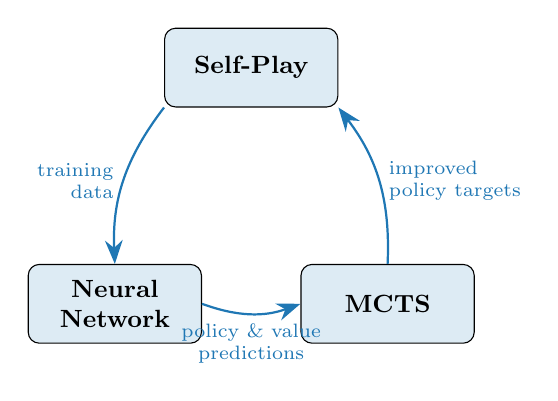
\begin{tikzpicture}[
  box/.style={draw, rounded corners, minimum width=2.2cm, minimum height=1cm,
              align=center, font=\small\bfseries, fill=azblue!15},
  arr/.style={-{Stealth[length=3mm]}, thick, azblue}
]
  \node[box] (sp) at (90:2.0) {Self-Play};
  \node[box] (nn) at (210:2.0) {Neural\\Network};
  \node[box] (mcts) at (330:2.0) {MCTS};

  \draw[arr] (sp.south west) to[bend right=20]
    node[midway, left, font=\scriptsize, align=right] {training\\data} (nn.north);
  \draw[arr] (nn.east) to[bend right=20]
    node[midway, below, font=\scriptsize, align=center] {policy \& value\\predictions} (mcts.west);
  \draw[arr] (mcts.north) to[bend right=20]
    node[midway, right, font=\scriptsize, align=left] {improved\\policy targets} (sp.south east);
\end{tikzpicture}
\end{column}
\end{columns}
\end{frame}

% ============================================================
% SLIDE 4: MCTS
% ============================================================
\begin{frame}{Monte Carlo Tree Search (MCTS)}
\begin{columns}[T]
\begin{column}{0.52\textwidth}
\textbf{Action selection via UCB:}
\[
  \text{UCB}(s,a) = \bar{Q}(s,a) + c \cdot \pi_\theta(a|s) \cdot \frac{\sqrt{N(s)}}{1 + N(s,a)}
\]

\vspace{0.2cm}
\textbf{Four phases per simulation:}
\begin{enumerate}
  \item \textbf{Select:} Follow UCB down the tree
  \item \textbf{Expand:} Add new leaf, query network for $(\pi, v)$
  \item \textbf{Backup:} Propagate $v$ up the path
  \item \textbf{Return:} Root visit counts $\to$ policy target
\end{enumerate}
\end{column}
\begin{column}{0.45\textwidth}
\vspace{0.3cm}
\textbf{Key insight:}\\[0.3cm]
The visit-count distribution at the root becomes the \alert{training target} for the policy head.

\vspace{0.5cm}
\textbf{Exploration:} Dirichlet noise added at root:
\[
  \pi'(a) = (1-\epsilon)\,\pi_\theta(a) + \epsilon\,\eta_a
\]
where $\eta \sim \text{Dir}(\alpha)$
\end{column}
\end{columns}
\end{frame}

% ============================================================
% SLIDE 5: Neural Network
% ============================================================
\begin{frame}{The Neural Network}
\begin{columns}[T]
\begin{column}{0.45\textwidth}
\centering
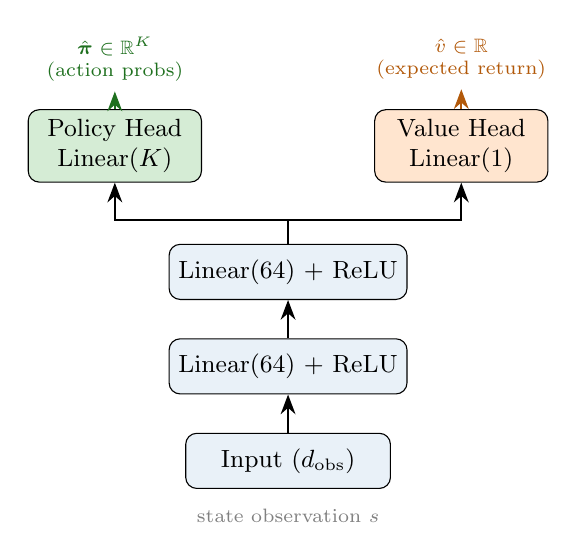
\begin{tikzpicture}[
  layer/.style={draw, rounded corners, minimum width=2.6cm, minimum height=0.7cm,
                align=center, font=\small, fill=azblue!10},
  head/.style={draw, rounded corners, minimum width=2.2cm, minimum height=0.7cm,
               align=center, font=\small},
  io/.style={font=\scriptsize, align=center},
  arr/.style={-{Stealth[length=2.5mm]}, thick}
]
  \node[layer] (input) at (0,0) {Input ($d_\text{obs}$)};
  \node[layer] (h1) at (0, 1.2) {Linear(64) + ReLU};
  \node[layer] (h2) at (0, 2.4) {Linear(64) + ReLU};

  \node[head, fill=azgreen!20] (policy) at (-2.2, 4.0) {Policy Head\\Linear($K$)};
  \node[head, fill=azorange!20] (value)  at ( 2.2, 4.0) {Value Head\\Linear(1)};

  \node[io, azgreen!70!black] (pout) at (-2.2, 5.1) {$\hat{\boldsymbol{\pi}} \in \mathbb{R}^K$\\(action probs)};
  \node[io, azorange!70!black] (vout) at ( 2.2, 5.1) {$\hat{v} \in \mathbb{R}$\\(expected return)};

  \node[io, gray] at (0, -0.7) {state observation $s$};

  \draw[arr] (input) -- (h1);
  \draw[arr] (h1) -- (h2);
  \draw[arr] (h2.north) -- ++(0,0.3) -| (policy.south);
  \draw[arr] (h2.north) -- ++(0,0.3) -| (value.south);
  \draw[arr, azgreen!70!black] (policy) -- (pout);
  \draw[arr, azorange!70!black] (value) -- (vout);
\end{tikzpicture}
\end{column}
\begin{column}{0.52\textwidth}
\textbf{Input:} state observation $s \in \mathbb{R}^{d_\text{obs}}$\\[0.15cm]
\textbf{Outputs:}
\begin{itemize}
  \item $\hat{\boldsymbol{\pi}}(\cdot|s)$: probability over $K$ actions
  \item $\hat{v}(s)$: predicted game return (scalar)
\end{itemize}

\vspace{0.3cm}
\textbf{Training targets} (from self-play):
\begin{itemize}
  \item $\boldsymbol{\pi}_\text{MCTS}$: MCTS visit-count distribution
  \item $z$: actual discounted return of the game
\end{itemize}

\vspace{0.3cm}
\textbf{Loss:}
\[
  \mathcal{L} = \underbrace{(\hat{v}(s) - z)^2}_{\substack{\text{value loss:}\\\text{predict game outcome}}}
              + \; 2 \cdot \underbrace{\text{CE}\bigl(\hat{\boldsymbol{\pi}},\, \boldsymbol{\pi}_\text{MCTS}\bigr)}_{\substack{\text{policy loss:}\\\text{match MCTS policy}}}
\]

\vspace{0.1cm}
{\small Adam, $\text{lr} = 3 \times 10^{-4}$, grad clip at norm 1.0}
\end{column}
\end{columns}
\end{frame}

% ############################################################
\section{The Doors Problem}
% ############################################################

% ============================================================
% SLIDE 6: Doors Setup
% ============================================================
\begin{frame}{The Doors Problem}
\begin{columns}[T]
\begin{column}{0.55\textwidth}
\centering
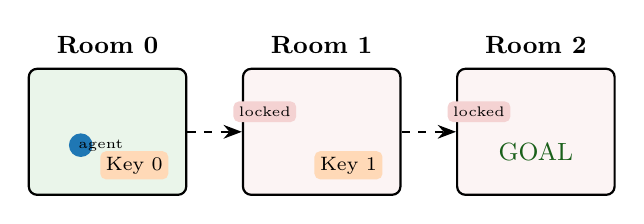
\begin{tikzpicture}[
  room/.style={draw, thick, minimum width=2.0cm, minimum height=1.6cm, rounded corners=3pt},
  key/.style={font=\scriptsize, fill=azorange!30, rounded corners=2pt, inner sep=2pt},
  lock/.style={font=\scriptsize, fill=failure!20, rounded corners=2pt, inner sep=2pt},
  agent/.style={circle, fill=azblue, minimum size=0.3cm, inner sep=0},
  scale=0.85
]
  % Room 0
  \node[room, fill=azgreen!10] (r0) at (0, 0) {};
  \node[above=0.05cm of r0, font=\small\bfseries] {Room 0};
  \node[agent] at (-0.4, -0.2) {};
  \node[font=\tiny] at (-0.1, -0.2) {agent};
  \node[key] at (0.4, -0.5) {\rotatebox{0}{Key 0}};

  % Room 1
  \node[room, fill=failure!5] (r1) at (3.2, 0) {};
  \node[above=0.05cm of r1, font=\small\bfseries] {Room 1};
  \node[lock] at (2.35, 0.3) {\tiny locked};
  \node[key] at (3.6, -0.5) {\rotatebox{0}{Key 1}};

  % Room 2
  \node[room, fill=failure!5] (r2) at (6.4, 0) {};
  \node[above=0.05cm of r2, font=\small\bfseries] {Room 2};
  \node[lock] at (5.55, 0.3) {\tiny locked};
  \node[font=\small, azgreen!60!black] at (6.4, -0.3) {GOAL};

  % Arrows
  \draw[-{Stealth}, thick, dashed] (r0.east) -- (r1.west);
  \draw[-{Stealth}, thick, dashed] (r1.east) -- (r2.west);
\end{tikzpicture}

\vspace{0.2cm}
{\small Example: $D=3$ rooms}
\end{column}
\begin{column}{0.42\textwidth}
\textbf{Actions:}
\begin{itemize}
  \item \texttt{MOVE\_TO}($\ell$) -- move to location
  \item \texttt{PICK}($k$) -- pick up key $k$
  \item \texttt{NOOP} -- do nothing
\end{itemize}

\vspace{0.2cm}
\textbf{Rewards:} $-0.01$/step, $+0.10$/unlock

\vspace{0.2cm}
\textbf{Observation:}\\
{\small One-hot location $+$ unlock status $+$ key availability}
\end{column}
\end{columns}

\vspace{0.3cm}
\textbf{Optimal plan for $D{=}3$ (5 steps):}\\[0.15cm]
\centering
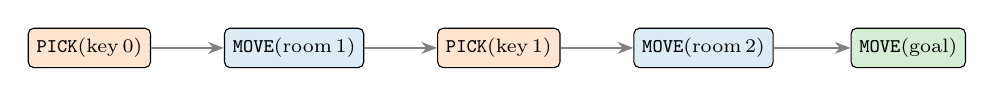
\begin{tikzpicture}[
  stp/.style={draw, rounded corners=2pt, font=\scriptsize, inner sep=3pt, minimum height=0.5cm},
  arr/.style={-{Stealth[length=2mm]}, thick, gray},
]
  \node[stp, fill=azorange!20] (s1) at (0,0) {\texttt{PICK}(key\,0)};
  \node[stp, fill=azblue!15]   (s2) at (2.6,0) {\texttt{MOVE}(room\,1)};
  \node[stp, fill=azorange!20] (s3) at (5.2,0) {\texttt{PICK}(key\,1)};
  \node[stp, fill=azblue!15]   (s4) at (7.8,0) {\texttt{MOVE}(room\,2)};
  \node[stp, fill=azgreen!20]  (s5) at (10.4,0) {\texttt{MOVE}(goal)};
  \draw[arr] (s1) -- (s2);
  \draw[arr] (s2) -- (s3);
  \draw[arr] (s3) -- (s4);
  \draw[arr] (s4) -- (s5);
\end{tikzpicture}

\vspace{0.15cm}
{\small General pattern: (\texttt{PICK} $\to$ \texttt{MOVE})$^{D-1}$ $\to$ \texttt{MOVE}(goal). Optimal length = $2(D{-}1)+1$ steps.}
\end{frame}

% ============================================================
% SLIDE 7: Why Doors is Hard
% ============================================================
\begin{frame}{Why Doors is Hard for AlphaZero}

\begin{enumerate}
  \item \textbf{No action masking:} $\sim$75--80\% of actions are \alert{silent no-ops}\\
    {\small Moving to a locked room or picking an unavailable key does nothing -- no negative signal, just wasted time.}

  \vspace{0.4cm}
  \item \textbf{Long sequential dependencies:} Must execute key$\to$unlock chain in strict order\\
    {\small $D=14$ requires a 27-step optimal plan. Every step must be correct.}

  \vspace{0.4cm}
  \item \textbf{Combinatorial action space:} $K = 4D$ total actions, but only $\sim$5--6 useful at any state\\
    {\small MCTS must discover the correct sequence by chance before the network can learn.}
\end{enumerate}

\vspace{0.4cm}
\begin{center}
\fcolorbox{azblue}{azblue!5}{\parbox{0.8\textwidth}{\centering
\textbf{Core challenge:} MCTS must explore deeply enough to see the key$\to$unlock reward chain (depth $\geq 2$) to produce useful policy targets.
}}
\end{center}
\end{frame}

% ============================================================
% SLIDE 8: Problem Dimensions
% ============================================================
\begin{frame}{Problem Dimensions}

\centering
\begin{tabular}{crrrrrc}
\toprule
$D$ & obs & actions ($K$) & opt.\ steps & horizon & net params & state space \\
\midrule
2 &  9 &  8 &  3 &  15 &  1{,}225 &       48 \\
3 & 14 & 12 &  5 &  25 &  1{,}805 &      288 \\
4 & 19 & 16 &  7 &  35 &  2{,}829 &    1{,}536 \\
5 & 24 & 20 &  9 &  45 &  4{,}437 &    7{,}680 \\
6 & 29 & 24 & 11 &  55 &  6{,}405 &   36{,}864 \\
\midrule
14 & 69 & 56 & 27 & 135 & $\sim$40K & $\sim 10^{10}$ \\
\bottomrule
\end{tabular}

\vspace{0.5cm}
State space grows \textbf{exponentially}; action count grows \textbf{linearly} with $D$.

\vspace{0.2cm}
{\small All experiments: \texttt{locs\_per\_room}=3, $T=1.0$, $c=1.5$, Dirichlet noise, no action masking, no gating.}

\end{frame}

% ############################################################
\section{The D=14 Failure}
% ############################################################

% ============================================================
% SLIDE 9: The Motivating Failure
% ============================================================
\begin{frame}{The Motivating Failure: D=14 Spike-and-Collapse}

\textbf{Configuration:} $D=14$, sims$=120$, games$=20$, 20 iterations

\vspace{0.3cm}
\begin{center}
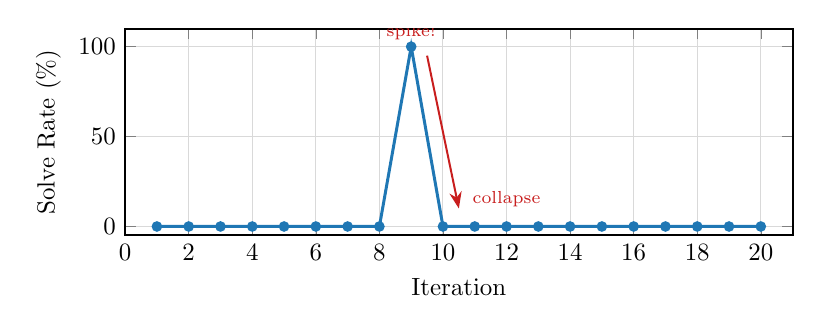
\begin{tikzpicture}[scale=0.9]
\begin{axis}[
  width=11cm, height=4.5cm,
  xlabel={Iteration}, ylabel={Solve Rate (\%)},
  xmin=0, xmax=21, ymin=-5, ymax=110,
  xtick={0,2,4,6,8,10,12,14,16,18,20},
  ytick={0,50,100},
  grid=major, grid style={gray!30},
  thick
]
\addplot[azblue, very thick, mark=*, mark size=1.5pt] coordinates {
  (1,0) (2,0) (3,0) (4,0) (5,0) (6,0) (7,0) (8,0)
  (9,100) (10,0) (11,0) (12,0) (13,0) (14,0) (15,0) (16,0) (17,0) (18,0) (19,0) (20,0)
};
\node[font=\scriptsize, failure] at (axis cs:9,108) {spike!};
\draw[-{Stealth}, failure, thick] (axis cs:9.5,95) -- (axis cs:10.5,10);
\node[font=\scriptsize, failure] at (axis cs:12,15) {collapse};
\end{axis}
\end{tikzpicture}
\end{center}

\vspace{0.1cm}
\begin{itemize}
  \item Iterations 1--8: 0\% solve rate. Policy loss $\approx 3.9$ (near $\ln 56 = 4.03$, i.e.\ uniform).
  \item Iteration 9: sudden spike to 100\%.
  \item Iteration 10+: immediate collapse, never recovers.
\end{itemize}
\end{frame}

% ============================================================
% SLIDE 10: Hypothesis
% ============================================================
\begin{frame}{Hypothesis: Data Starvation}

\textbf{Prior successful D=14 runs} used \texttt{games=50}.\\
This run used \texttt{games=20} -- 2.5$\times$ less data.

\vspace{0.4cm}
\begin{columns}[T]
\begin{column}{0.48\textwidth}
\textbf{The numbers:}
\begin{itemize}
  \item games$=20$, horizon$=135$
  \item $\Rightarrow \sim$2{,}700 examples/iteration
  \item Network has $\sim$40K parameters
  \item Buffer at iter 10: $\sim$27K examples
  \item Ratio: $\sim$0.7$\times$ params
\end{itemize}
\end{column}
\begin{column}{0.48\textwidth}
\textbf{The mechanism:}
\begin{itemize}
  \item Network overfits each small batch
  \item Destroys previously learned weights
  \item Spike = one lucky iteration
  \item Collapse = catastrophic forgetting
\end{itemize}
\end{column}
\end{columns}

\vspace{0.5cm}
\begin{center}
\fcolorbox{azblue}{azblue!5}{\parbox{0.85\textwidth}{\centering
\textbf{Question:} Can we reproduce this failure at small scale\\and map the exact thresholds?
}}
\end{center}
\end{frame}

% ############################################################
\section{Systematic Small-Scale Verification}
% ############################################################

% ============================================================
% SLIDE 11: Experimental Design
% ============================================================
\begin{frame}{Experimental Design}

\textbf{13 runs} across four experiment groups:

\vspace{0.3cm}
\centering
\begin{tabular}{clll}
\toprule
Group & Question & Sweep variable & Fixed \\
\midrule
\textbf{A} & Does the code work? & $D \in \{2, 3\}$ & sims=25, games=20 \\
\textbf{B} & How much search? & sims $\in \{5, 10, 25, 50\}$ & $D=4$, games=20 \\
\textbf{C} & How much data? & games $\in \{5, 10, 20, 40\}$ & $D=4$, sims=25 \\
\textbf{D} & How does difficulty scale? & $D \in \{2, 3, 4, 5, 6\}$ & sims=25, games=20 \\
\bottomrule
\end{tabular}

\vspace{0.5cm}
\textbf{All experiments held constant:}\\
{\small $T{=}1.0$, $c{=}1.5$, Dir$(\alpha{=}0.25, \epsilon{=}0.4)$, replay buffer = 20 iters, no gating, no masking, 8 parallel workers.}
\end{frame}

% ============================================================
% SLIDE 12: Experiment A
% ============================================================
\begin{frame}{Experiment A: Sanity Check}

\textbf{Settings:} sims$=25$, games$=20$, 15 iterations.

\vspace{0.4cm}
\centering
\begin{tabular}{clll}
\toprule
$D$ & First solve & Optimal by & Stable? \\
\midrule
2 & iter 1 & iter 4 & \textcolor{success}{Yes -- 100\% all 15 iterations} \\
3 & iter 3 & iter 7 & \textcolor{success}{Yes -- 100\% from iter 3 onward} \\
\bottomrule
\end{tabular}

\vspace{0.6cm}
\begin{center}
\fcolorbox{success}{success!8}{\parbox{0.75\textwidth}{\centering
\textbf{Verdict: The code is correct.}\\[0.2cm]
$D{=}2$ solves from iteration 1 (MCTS alone finds the 3-step plan with a random network).\\
$D{=}3$ converges cleanly by iteration 7.
}}
\end{center}
\end{frame}

% ============================================================
% SLIDE 13: Experiment B
% ============================================================
\begin{frame}{Experiment B: MCTS Simulation Sweep ($D{=}4$)}

\centering
\begin{tabular}{rrllp{4.5cm}}
\toprule
sims & sims/$K$ & First solve & Outcome & \\
\midrule
  5 & 0.31 & iter 19     & \textcolor{fragile}{Spike-collapse} & Brief spike then anti-learning \\
 10 & 0.63 & never       & \textcolor{failure}{Dead}            & 0\% all 30 iterations \\
 25 & 1.56 & iter 2      & \textcolor{success}{Stable}          & Optimal by iter 13 \\
 50 & 3.12 & iter 1      & \textcolor{success}{Stable}          & MCTS alone solves \\
\bottomrule
\end{tabular}

\vspace{0.5cm}
\begin{itemize}
  \item \textbf{Sharp threshold} between sims/$K = 0.63$ (dead) and $1.56$ (stable)
  \item \textbf{Counterintuitive:} sims$=10$ is \emph{worse} than sims$=5$
    \begin{itemize}
      \item[\scriptsize$\bullet$] {\small At sims$=5$: tree occasionally stumbles into rewarding branch}
      \item[\scriptsize$\bullet$] {\small At sims$=10$: visits spread uniformly but not enough to differentiate $\to$ maximally uninformative targets}
    \end{itemize}
\end{itemize}
\end{frame}

% ============================================================
% SLIDE 14: Why the Threshold is Sharp
% ============================================================
\begin{frame}{Why the MCTS Threshold is Sharp}

\begin{columns}[T]
\begin{column}{0.48\textwidth}
\textbf{Below threshold} (sims/$K < 1$):
\begin{itemize}
  \item With random network, visits spread roughly uniformly across $K$ actions
  \item Most actions get 0 or 1 visit
  \item Visit counts are \alert{noise}
  \item Network trains on garbage
  \item No learning signal at all
\end{itemize}
\end{column}
\begin{column}{0.48\textwidth}
\textbf{Above threshold} (sims/$K \geq 1.5$):
\begin{itemize}
  \item Enough visits for UCB to \textbf{differentiate} good from bad actions
  \item Tree reaches depth $\geq 2$: sees key$\to$unlock reward chain
  \item Visit counts carry \textbf{real signal}
  \item Network improves, MCTS improves
  \item Virtuous cycle engages
\end{itemize}
\end{column}
\end{columns}

\vspace{0.5cm}
\begin{center}
\fcolorbox{azblue}{azblue!5}{\parbox{0.8\textwidth}{\centering
The transition from ``random noise'' to ``useful signal'' happens in a \textbf{narrow band} around sims/$K \approx 1$.
}}
\end{center}
\end{frame}

% ============================================================
% SLIDE 15: Experiment C
% ============================================================
\begin{frame}{Experiment C: Data Volume Sweep ($D{=}4$, sims$=25$)}

\centering
\begin{tabular}{rrrll}
\toprule
games & ex./iter & buffer/params & First solve & Outcome \\
\midrule
  5 & $\sim$175   & 0.6$\times$  & iter 3 & \textcolor{failure}{Spike-and-collapse (10 collapses in 30 iters)} \\
 10 & $\sim$350   & 1.2$\times$  & iter 3 & \textcolor{success}{Stable, optimal by iter 22} \\
 20 & $\sim$700   & 2.5$\times$  & iter 2 & \textcolor{success}{Stable, optimal by iter 13} \\
 40 & $\sim$1{,}400 & 5.0$\times$  & iter 1 & \textcolor{success}{Stable, optimal by iter 2} \\
\bottomrule
\end{tabular}

\vspace{0.2cm}
{\footnotesize Buffer/params measured at iteration 10. Network has 2{,}829 parameters.}

\vspace{0.5cm}
\begin{center}
\fcolorbox{failure}{failure!8}{\parbox{0.85\textwidth}{\centering
\textbf{Key result:} \texttt{games=5} at $D{=}4$ reproduces the $D{=}14$ failure pattern \emph{exactly}.\\[0.15cm]
Threshold: replay buffer $\geq 1.2\times$ network parameters for stable learning.
}}
\end{center}
\end{frame}

% ============================================================
% SLIDE 16: Spike-and-Collapse Mechanism
% ============================================================
\begin{frame}{The Spike-and-Collapse Mechanism}

\centering
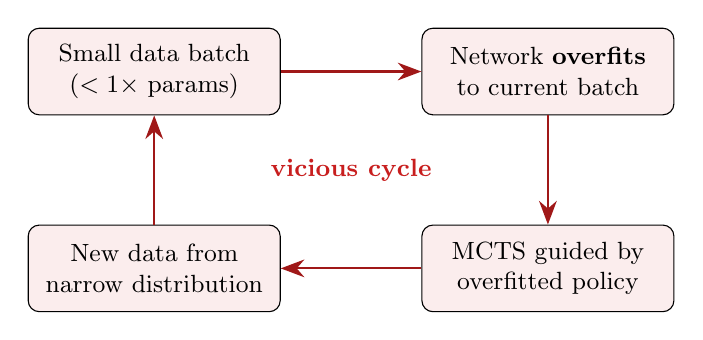
\begin{tikzpicture}[
  box/.style={draw, rounded corners, minimum width=3.2cm, minimum height=1.1cm,
              align=center, font=\small, fill=failure!8},
  arr/.style={-{Stealth[length=3mm]}, thick, failure!80!black},
  node distance=0.6cm
]
  \node[box] (a) at (0, 0) {Small data batch\\($< 1\times$ params)};
  \node[box] (b) at (5, 0) {Network \textbf{overfits}\\to current batch};
  \node[box] (c) at (5, -2.5) {MCTS guided by\\overfitted policy};
  \node[box] (d) at (0, -2.5) {New data from\\narrow distribution};

  \draw[arr] (a) -- (b);
  \draw[arr] (b) -- (c);
  \draw[arr] (c) -- (d);
  \draw[arr] (d) -- (a);

  \node[font=\small\bfseries, failure] at (2.5, -1.25) {vicious cycle};
\end{tikzpicture}

\vspace{0.4cm}
\begin{columns}[T]
\begin{column}{0.45\textwidth}
\centering
\textbf{Train reward:} stays high\\
{\small (network fits its training data well)}
\end{column}
\begin{column}{0.45\textwidth}
\centering
\textbf{Eval reward:} crashes\\
{\small (policy does not generalize)}
\end{column}
\end{columns}
\end{frame}

% ============================================================
% SLIDE 17: Experiment D
% ============================================================
\begin{frame}{Experiment D: Difficulty Scaling (sims$=25$, games$=20$)}

\centering
\begin{tabular}{rrlll}
\toprule
$D$ & sims/$K$ & First solve & Outcome & Regime \\
\midrule
2 & 3.12 & iter 1  & \textcolor{success}{Stable, optimal}   & \textcolor{success}{Comfortable} \\
3 & 2.08 & iter 3  & \textcolor{success}{Stable, optimal}   & \textcolor{success}{Comfortable} \\
4 & 1.56 & iter 2  & \textcolor{success}{Stable, optimal by iter 13} & \textcolor{success}{Comfortable} \\
5 & 1.25 & iter 2  & \textcolor{fragile}{Collapsed at iter 26} & \textcolor{fragile}{Fragile} \\
6 & 1.04 & iter 32 & \textcolor{azblue}{Slow bootstrap, then stable} & \textcolor{azblue}{Slow bootstrap} \\
\bottomrule
\end{tabular}

\vspace{0.5cm}
Three distinct regimes emerge as sims/$K$ decreases:

\vspace{0.2cm}
\begin{description}
  \item[\textcolor{success}{Comfortable}] (sims/$K \geq 1.5$): Fast, stable learning
  \item[\textcolor{fragile}{Fragile}] (sims/$K \approx 1.25$): Learns, then collapses -- \alert{most dangerous}
  \item[\textcolor{azblue}{Slow bootstrap}] (sims/$K \approx 1.0$): Long plateau, then sudden breakthrough
\end{description}
\end{frame}

% ============================================================
% SLIDE 18: Three Regimes Plot
% ============================================================
\begin{frame}{Three Regimes: Conceptual Picture}

\centering
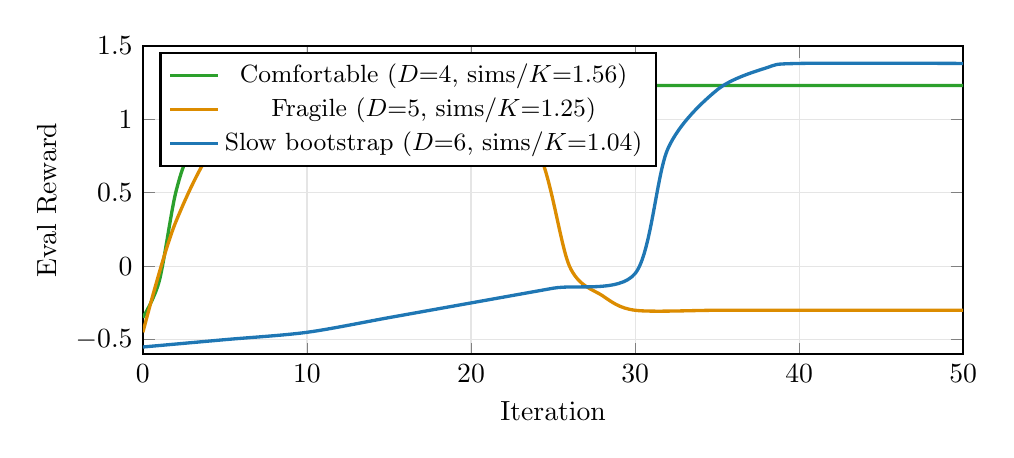
\begin{tikzpicture}
\begin{axis}[
  width=12cm, height=5.5cm,
  xlabel={Iteration}, ylabel={Eval Reward},
  xmin=0, xmax=50, ymin=-0.6, ymax=1.5,
  xtick={0,10,20,30,40,50},
  grid=major, grid style={gray!20},
  legend style={at={(0.02,0.98)}, anchor=north west, font=\small},
  thick
]

% Comfortable (D=4): rises quickly, stays flat
\addplot[azgreen, very thick, smooth] coordinates {
  (0,-0.35) (1,-0.1) (2,0.5) (3,0.8) (5,1.0) (8,1.15) (13,1.23) (20,1.23) (30,1.23) (40,1.23) (50,1.23)
};
\addlegendentry{Comfortable ($D{=}4$, sims/$K{=}1.56$)}

% Fragile (D=5): rises, then crashes
\addplot[fragile, very thick, smooth] coordinates {
  (0,-0.45) (2,0.3) (5,0.9) (10,1.1) (15,1.2) (20,1.1) (24,0.8) (26,0.0) (28,-0.2) (30,-0.3) (35,-0.3) (40,-0.3) (50,-0.3)
};
\addlegendentry{Fragile ($D{=}5$, sims/$K{=}1.25$)}

% Slow bootstrap (D=6): flat for long, then jumps
\addplot[azblue, very thick, smooth] coordinates {
  (0,-0.55) (5,-0.5) (10,-0.45) (15,-0.35) (20,-0.25) (25,-0.15) (30,-0.05) (32,0.8) (35,1.2) (38,1.35) (40,1.38) (50,1.38)
};
\addlegendentry{Slow bootstrap ($D{=}6$, sims/$K{=}1.04$)}

\end{axis}
\end{tikzpicture}

\vspace{0.2cm}
\textbf{Paradox:} $D{=}5$ (easier) fails while $D{=}6$ (harder) succeeds.\\
{\small $D{=}5$ learns fast enough to overshoot into a bad local minimum.\\$D{=}6$ improves so gradually it never overshoots.}
\end{frame}

% ############################################################
\section{Diagnosis and Conclusions}
% ############################################################

% ============================================================
% SLIDE 19: D=14 Diagnosis
% ============================================================
\begin{frame}{Diagnosing the D=14 Failure}

\begin{columns}[T]
\begin{column}{0.48\textwidth}
\textbf{MCTS budget: adequate}
\begin{itemize}
  \item sims/$K = 120/56 = 2.14$
  \item Well within ``comfortable'' regime
  \item Prior D=14 runs with sims$=120$ succeeded
\end{itemize}

\vspace{0.3cm}
\textbf{Data volume: \alert{insufficient}}
\begin{itemize}
  \item games$=20$, horizon$=135$
  \item $\sim$2{,}700 examples/iter
  \item 27-step plan: each example covers one state
  \item Effective coverage is thin
\end{itemize}
\end{column}
\begin{column}{0.48\textwidth}
\vspace{0.2cm}
\begin{center}
\fcolorbox{success}{success!8}{\parbox{0.9\textwidth}{\centering
\textbf{Root cause confirmed:}\\[0.2cm]
Data starvation,\\not a code bug.\\[0.3cm]
\textbf{Fix:} increase\\games $20 \to 50$
}}
\end{center}

\vspace{0.3cm}
{\small The spike-and-collapse at D=14 (iter 9$\to$10) matches the games=5 failure at D=4 exactly.}
\end{column}
\end{columns}
\end{frame}

% ============================================================
% SLIDE 20: Summary of Thresholds
% ============================================================
\begin{frame}{Summary of Thresholds}

\centering
\begin{tabular}{lll}
\toprule
\textbf{Quantity} & \textbf{Threshold} & \textbf{Evidence} \\
\midrule
MCTS budget    & sims/$K \geq 1.5$         & sims/$K{=}0.63$ dead, $1.56$ stable \\[0.3cm]
Data volume    & buffer $\geq 1.2\times$ params & games$=5$ unstable, games$=10$ stable \\[0.3cm]
Difficulty     & 3 regimes                 & Comfortable / Fragile / Slow bootstrap \\
\bottomrule
\end{tabular}

\vspace{0.7cm}
\begin{center}
\fcolorbox{azblue}{azblue!5}{\parbox{0.85\textwidth}{\centering
\textbf{The single most important result:}\\[0.2cm]
\texttt{games=5} at $D{=}4$ reproduces the $D{=}14$ failure pattern (spike-and-collapse) at small scale. This confirms \textbf{data starvation} -- not a code bug -- as the root cause.
}}
\end{center}
\end{frame}

% ============================================================
% SLIDE 21: Lessons and Next Steps
% ============================================================
\begin{frame}{Lessons and Next Steps}

\textbf{Lessons:}
\begin{enumerate}
  \item AlphaZero has \textbf{sharp phase transitions} in both search budget and data volume
  \item The ``fragile'' regime is the most dangerous: \alert{looks like success before it collapses}
  \item Small-scale reproduction of large-scale failures is a powerful diagnostic tool
\end{enumerate}

\vspace{0.5cm}
\textbf{Next steps:}
\begin{enumerate}
  \item Rerun D=14 with games$=50$, sims$=120$, iters$=40$
  \item Investigate \textbf{acceptance gating} as a stabilizer for the fragile regime
  \item Scale to larger $D$ with budget rules: sims $\geq 1.5K$, buffer $\geq 2\times$ params
  \item Explore \textbf{action masking} to reduce effective action space
\end{enumerate}
\end{frame}

% ============================================================
% SLIDE 22: Thank You
% ============================================================
\begin{frame}{}
\centering
\vspace{2cm}
{\Huge Thank You}

\vspace{1cm}
{\Large Questions?}

\vspace{1.5cm}
{\small All experiments and code available at:\\
\texttt{AlphaZero\_PP/experiments/doors\_direct/}}
\end{frame}

\end{document}
